\documentclass[12pt]{article}
\usepackage{a4,fancyhdr,moreverb,epsfig,amssymb,amsmath,ifthen}
\usepackage[utf8]{inputenc}
\usepackage[english]{babel}
\usepackage{mathtools}
\usepackage{lstautogobble}
\usepackage[framed,numbered]{mcode}
\usepackage{listings}
\usepackage{subcaption}
\usepackage{amsthm}
\textwidth 455pt \oddsidemargin 0mm
\parindent 12pt
\textheight 685pt % old : 665pt
\textheight 697pt
\topmargin -40pt  % old -70pt
\newcommand{\cpp}{C\raisebox{.4ex}{\tiny ++}}
\renewcommand{\vec}{\underline}
\newcommand{\va}{\underline{a}}
\newcommand{\vb}{\underline{b}}
\newcommand{\vc}{\underline{c}}
\newcommand{\vh}{\underline{h}}
\newcommand{\ve}{\underline{e}}
\newcommand{\vg}{\underline{g}}
\newcommand{\vp}{\underline{p}}
\newcommand{\vq}{\underline{q}}
\newcommand{\vu}{\underline{u}}
\newcommand{\vv}{\underline{v}}
\newcommand{\vw}{\underline{w}}
\newcommand{\vx}{\underline{x}}
\newcommand{\vy}{\underline{y}}
\newcommand{\vz}{\underline{z}}
\newcommand\myeq{\stackrel{\mathclap{\normalfont\mbox{cgs}}}{=}}
\newcommand{\dd}[1]{\mathrm{d}#1}


\usepackage{graphicx}
\graphicspath{ {./images/} }


\begin{document}
\pagestyle{fancyplain}
\lhead{\fancyplain{}{\sf M4S18B2 Machine Learning}}
\rhead{\fancyplain{}{\sf Omar Haque}}
\cfoot{}{}


\begin{center} \Large
Machine Learning - Coursework 1 \\[4mm]
\end{center}

\par \hfill\hrulefill\hfill \vspace{2mm}


\vspace{0.3in}

\begin{itemize}
\item \textbf{Calculate and plot the average face of the training set, then write a function to find a PCA basis of size M, where the inputs will be M and X, the matrix containing the training set. Clearly describe all aspects of your function, then use it to plot the first 5 eigenfaces of the training set.}
\end{itemize}

To calculate the average face of the training set, I simply calculate the average pixel values for each pixel across the trainings set.

\begin{lstlisting}[linewidth=18.4cm,language=R]
library(rARPACK)
library(philentropy)


# I load the raw csv's
faces.train.inputs <- read.csv("./2018_ML_Assessed_Coursework_1_Data/
                               Faces_Train_Inputs.csv",head=FALSE)
faces.train.label <- read.csv("./2018_ML_Assessed_Coursework_1_Data/
                              Faces_Train_Labels.csv",head=FALSE)
faces.test.inputs <- read.csv("./2018_ML_Assessed_Coursework_1_Data/
                              Faces_Test_Inputs.csv",head=FALSE)
faces.test.label <- read.csv("./2018_ML_Assessed_Coursework_1_Data/
                             Faces_Test_Labels.csv",head=FALSE)


# I turn the input values into a list of 320 matrices, each matrix a 112 x 92 value 
# of pixels corresponding to each image .. I need to use lapply again on the 
#result because apply gives the matrices in a weird form
faces.train.inputs.cleaned <- lapply(apply(X=faces.train.inputs, 
                                           MARGIN=1, 
                                           function(x) list(matrix(as.numeric(x), 
                                           nrow = 112))), "[[", 1)

# Here I calculate the average face
avg.face <- Reduce('+', faces.train.inputs.cleaned) / 
  length(faces.train.inputs.cleaned)
image(avg.face)
\end{lstlisting}

\newpage
\begin{figure}
\caption{Average face of the training set}
\centering
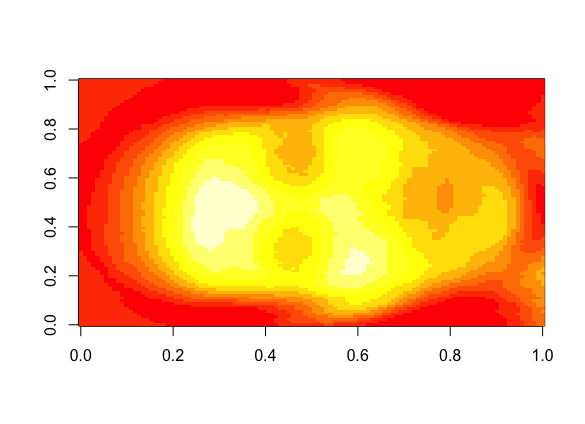
\includegraphics[width=0.5\textwidth]{average}
\end{figure}

The following function returns the PCA basis of size M as specified. I added a default parameter which also allows access to the eigenvalues associated with each vector of the eigenbasis.

The function works exactly as the PCA described in lectures. Calculate the centralised data matrix, $X$, and then calculate the first M eigenvectors for the covariance matrix $\frac{XX^{T}}{n}$.

\begin{lstlisting}[linewidth=18.4cm,language=R]
find.pca.basis <- function(M,X, return.full.results = FALSE){

  n <- dim(X)[1] # The number of images
  
  # Turn the input data into a matrix and transpose it
  X.data.matrix <- data.matrix(t(X))
  
  # Centralise the data matrix
  means <- rowMeans(X.data.matrix) # calculate row means
  data.matrix.centralised <- X.data.matrix - means %*% t(rep(1,n)) # and subtract
  
  # Calculate the covariance matrix as defined in lectures
  covariance.matrix <- (data.matrix.centralised %*% t(data.matrix.centralised)) / n
  
  # Now I need to compute the first M eigenvectors/ eigenvalues using the 
  # R package rARPACK
  results <- eigs_sym(covariance.matrix,k=M,which="LM")
  
  if (return.full.results){
    return(results)
  } else{
    return(results$vectors)
  }
  
}
\end{lstlisting}

\newpage
The code below then plots the first 5 eigenfaces of the training set. This means simply calculating the eigenbasis for M = 5, and then plotting the vectors in the resulting eigenbasis.
\begin{lstlisting}[linewidth=18.4cm,language=R]
eigenbasis <- find.pca.basis(5,faces.train.inputs)

par(mfrow=c(2,3))
for (i in 1:5){
  # eigenbasis[,i] corresponds to the i'th eigenvector.
  image(matrix(eigenbasis[,i], nrow = 112),useRaster=TRUE, axes=FALSE,main=i)
}
par(mfrow=c(1,1))
\end{lstlisting}

The results can be seen in figure 2.

\begin{figure}
\caption{First 5 Eigenfaces of the  training set}
\centering
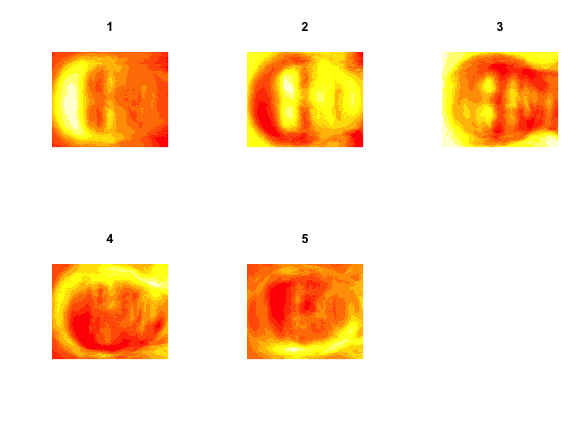
\includegraphics[width=0.8\textwidth]{eigenface}
\end{figure}


\begin{itemize}
\item \textbf{Choose a single face and project it into a PCA basis for dimension M = 5, 10, 50, then plot the results.}
\end{itemize}

Here is the code to project the first image of the training set onto the PCA basis for dimensions 5,10 and 50.
\newpage 
\begin{lstlisting}[linewidth=18.4cm,language=R]
# initialise the dimensions and face used.
dimensions <- c(5,10,50)
single.face <- 1
means <- as.vector(avg.face) # convert the mean face back into a vector

# iterate through the dimensions considered
for (i in dimensions){
  
  # compute the eigenbasis using the function created
  eigenbasis <- find.pca.basis(i,faces.train.inputs)
  # calculate the projection values in this pca basis
  projection.vals <- t(as.numeric(faces.train.inputs[single.face,]) - 
                         means) %*% eigenbasis
  # calculate the actual face in this basis
  projection.vector <- eigenbasis %*% as.numeric(as.list(projection.vals))
  
  # carry out the plot
  image(matrix(projection.vector, nrow = 112),useRaster=TRUE, 
        axes=FALSE,main=paste("dimension",i,sep=" "))
}

# and here's the original image
image(matrix(as.numeric(faces.train.inputs[single.face,]), nrow = 112), 
      useRaster=TRUE, axes=FALSE, main="Original Image")
\end{lstlisting}
Please see Figure 3 for the results of this code.

\begin{itemize}
\item \textbf{Plot a graph of the mean squared error of each lower dimensional approximation of this chosen face, with the dimensionality plotted along the x-axis. Is there a clear point at which we can choose a good approximation? Discuss how we should choose the appropriate dimensionality of the approximation.}
\end{itemize}

\newpage

    \begin{figure*}[t!]
        \centering
        \begin{subfigure}[b]{0.475\textwidth}
            \centering
            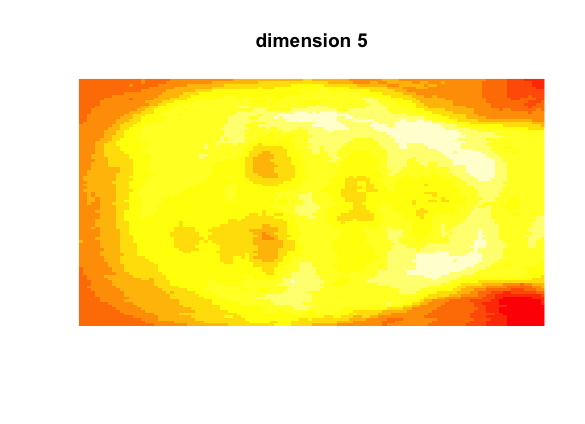
\includegraphics[width=\textwidth]{5}
            \caption[Dimension 5]%

            \label{fig:mean and std of net14}
        \end{subfigure}
        \hfill
        \begin{subfigure}[b]{0.475\textwidth}  
            \centering 
            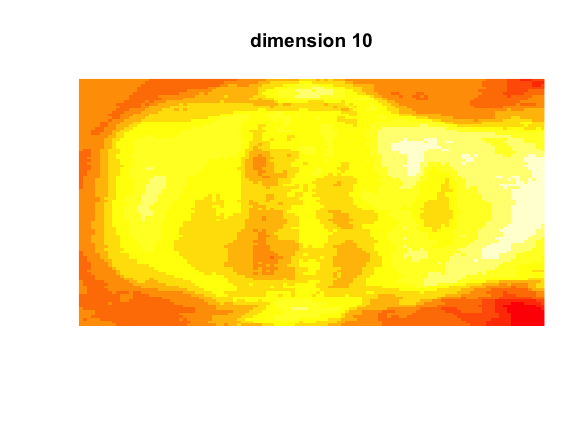
\includegraphics[width=\textwidth]{10}
            \caption[]%

            \label{fig:mean and std of net24}
        \end{subfigure}
        \vskip\baselineskip
        \begin{subfigure}[b]{0.475\textwidth}   
            \centering 
            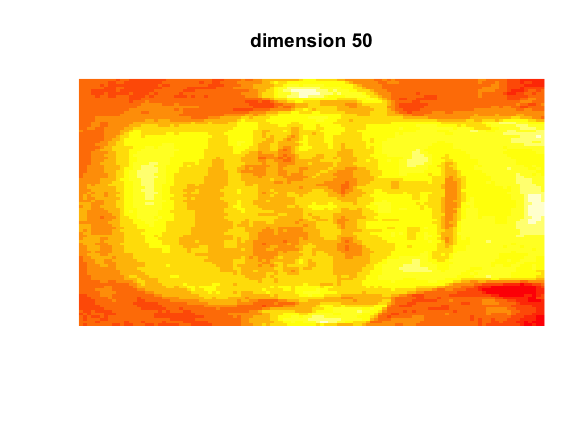
\includegraphics[width=\textwidth]{50}
            \caption[]%

            \label{fig:mean and std of net34}
        \end{subfigure}
        \quad
        \begin{subfigure}[b]{0.475\textwidth}   
            \centering 
            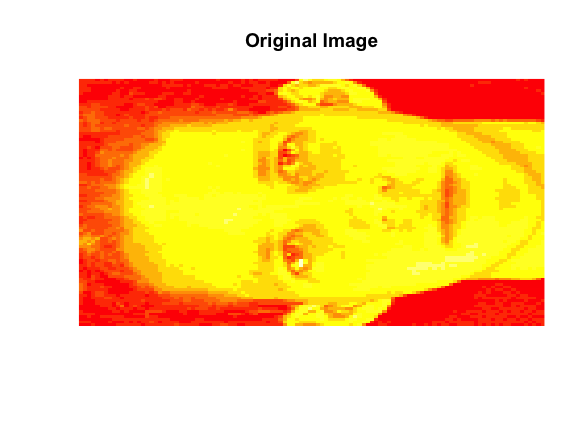
\includegraphics[width=\textwidth]{orig}
            \caption[]%
 
            \label{fig:mean and std of net44}
        \end{subfigure}
        \caption[ The average and standard deviation of critical parameters ]
        {\small The projection of training image 1 onto PCA bases of different dimensions} 
        \label{fig:mean and std of nets}
    \end{figure*}

\end{document}
